% Shared preamble for the CAWASMA viva notes (Atta, Asim, Neelam).
\documentclass[11pt,a4paper]{article}
\usepackage[T1]{fontenc}
\usepackage[utf8]{inputenc}
\usepackage{lmodern}
\usepackage{amsmath}
\usepackage{amssymb}
\usepackage{microtype}
\usepackage[margin=2.3cm]{geometry}
\usepackage{booktabs}
\usepackage{array}
\usepackage{tabularx}
\usepackage{longtable}
\usepackage{xcolor}
\usepackage{enumitem}
\usepackage{caption}
\usepackage{listings}
\usepackage{tikz}
\usetikzlibrary{arrows.meta,positioning,fit,backgrounds,calc}
\usepackage[hidelinks]{hyperref}

\definecolor{brand}{HTML}{1F4E79}
\definecolor{soft}{HTML}{F3F6F9}
\definecolor{rule}{HTML}{B8C2CC}
\definecolor{codebg}{HTML}{F7F8FA}
\definecolor{kw}{HTML}{1F5FA8}
\definecolor{cm}{HTML}{6A7684}

\captionsetup{font=small,labelfont={bf,color=brand},justification=raggedright,singlelinecheck=false}
\setlist{itemsep=2pt,topsep=3pt,parsep=0pt}
\sloppy
\hbadness=6000
\renewcommand{\arraystretch}{1.18}

% Code excerpts: small, wrapping, no language assumptions.
\lstset{
  basicstyle=\ttfamily\footnotesize,
  backgroundcolor=\color{codebg},
  frame=single, rulecolor=\color{rule},
  breaklines=true, breakatwhitespace=false,
  keywordstyle=\color{kw}\bfseries,
  commentstyle=\color{cm}\itshape,
  showstringspaces=false,
  columns=fullflexible,
  xleftmargin=6pt, xrightmargin=6pt,
  aboveskip=6pt, belowskip=6pt,
  literate={->}{{$\rightarrow$}}1 {<-}{{$\leftarrow$}}1,
}
\lstdefinestyle{py}{language=Python}

% Source footnote: where a fact came from in the repo.
\newcommand{\src}[1]{\footnote{Source: \texttt{#1}}}

% Person title block. \setperson{Name}{Role}{Roll}
\newcommand{\PersonName}{} \newcommand{\PersonRole}{} \newcommand{\PersonRoll}{}
\newcommand{\setperson}[3]{\renewcommand{\PersonName}{#1}\renewcommand{\PersonRole}{#2}\renewcommand{\PersonRoll}{#3}}

\newcommand{\maketitlepage}{%
\begin{titlepage}
\centering
\vspace*{1.2cm}
{\color{brand}\rule{\linewidth}{1.2pt}}\\[4mm]
{\Large\bfseries CAWASMA}\\[2mm]
{\large Context-Aware Web \& API Security Misconfiguration Analyzer}\\[3mm]
{\color{brand}\rule{\linewidth}{1.2pt}}\\[1.4cm]
{\large Final-year project --- viva study notes}\\[1.2cm]
{\Huge\bfseries \PersonName}\\[5mm]
{\large \PersonRole}\\[3mm]
{\large Roll number: \PersonRoll}\\[1.4cm]
\begin{tabular}{rl}
Supervisor: & Dr.\ Bilal Khan\\[2mm]
Team: & Asim Shakeel (22P-9229)\\
 & Neelam Jabeen (22P-9353)\\
 & Atta Ur Rehman (22P-9236)\\
\end{tabular}\\[1.2cm]
{\color{cm}\small These notes are generated from the repository, documentation and git history.\\
Every number is cited to the file or command it came from. Date: \today.}\\[1cm]
{\color{brand}\rule{\linewidth}{0.6pt}}
\end{titlepage}}

% A small helper for the "scoring in one line" boxes.
\newcommand{\keybox}[1]{\par\vspace{3pt}\noindent\fcolorbox{rule}{soft}{\parbox{\dimexpr\linewidth-2\fboxsep-2\fboxrule}{#1}}\par\vspace{3pt}}

\setperson{Asim Shakeel}{Check specs, CVSS mapping, ML \& evaluation}{22P-9229}
\begin{document}
\maketitlepage
\tableofcontents
\clearpage

% Part A: the whole project. Shared, identical in all three documents.
\section{The whole project}

\subsection{The problem}
A normal security scanner gives a fixed severity to each kind of finding. A
missing \texttt{X-Content-Type-Options} header is ``medium'' wherever it is
found: on a public brochure page, and on a login API that returns credentials.
The person reading the report then has to work out, by hand, which of a hundred
``medium'' findings actually matters. That triage is slow and easy to get
wrong. Tools such as OWASP ZAP and Nuclei do find real issues, but they rate
the issue, not the place it sits in.\src{docs/supervisor/scanners.md}

\subsection{The idea}
CAWASMA scores the \emph{same} finding differently according to where it occurs
and what the endpoint returned. It does this with the standard CVSS v3.1
\emph{environmental} metrics, so the result is not an invented number: it is a
recomputation of the official score with a vector anyone can check on the FIRST
calculator.

\keybox{\textbf{One-paragraph pitch.} CAWASMA is a defensive, black-box,
HTTPS-only scanner for web apps and REST APIs. Each of its checks carries a
fixed CVSS v3.1 base vector. For every finding it works out how sensitive the
endpoint is (from the URL path) and what sensitive data the response holds
(credentials, personal data, financial data, internal IPs). It turns those into
CVSS environmental security requirements (CR/IR/AR) and recomputes the score, so
a login API and a public page that share a weakness no longer share a priority.
The point of the project is \emph{prioritisation, not detection}.}

\subsection{Architecture}
A scan is a pipeline. A URL goes in; a ranked, explained report comes out.

\begin{center}
\resizebox{0.98\linewidth}{!}{%
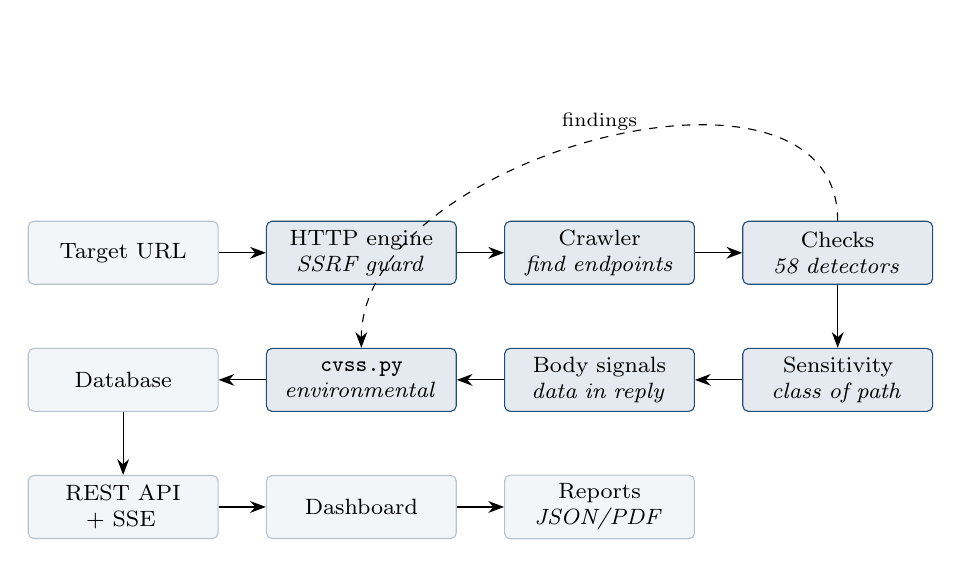
\begin{tikzpicture}[
  font=\footnotesize,
  >={Stealth[length=2mm]},
  box/.style={draw=rule,fill=soft,rounded corners=2pt,minimum height=8mm,inner sep=3pt,text width=22mm,align=center},
  core/.style={box,fill=brand!12,draw=brand},
  node distance=4mm and 6mm,
]
\node[box] (url) {Target URL};
\node[core,right=of url] (eng) {HTTP engine\\\textit{SSRF guard}};
\node[core,right=of eng] (crawl) {Crawler\\\textit{find endpoints}};
\node[core,right=of crawl] (checks) {Checks\\\textit{58 detectors}};
\node[core,below=8mm of checks] (sens) {Sensitivity\\\textit{class of path}};
\node[core,left=of sens] (body) {Body signals\\\textit{data in reply}};
\node[core,left=of body] (cvss) {\texttt{cvss.py}\\\textit{environmental}};
\node[box,left=of cvss] (db) {Database};
\node[box,below=8mm of db] (api) {REST API\\+ SSE};
\node[box,right=of api] (ui) {Dashboard};
\node[box,right=of ui] (rep) {Reports\\\textit{JSON/PDF}};
\draw[->] (url)--(eng); \draw[->] (eng)--(crawl); \draw[->] (crawl)--(checks);
\draw[->] (checks)--(sens); \draw[->] (sens)--(body); \draw[->] (body)--(cvss);
\draw[->] (cvss)--(db); \draw[->] (db)--(api); \draw[->] (api)--(ui); \draw[->] (ui)--(rep);
\draw[->,dashed] (checks.north) to[out=90,in=90] node[above,font=\scriptsize]{findings} (cvss.north);
\end{tikzpicture}}
\end{center}

\noindent The stages are: the \textbf{engine} fetches safely (one SSRF check per
redirect hop); the \textbf{crawler} discovers endpoints (seed, HTML, JavaScript,
a wordlist, and OpenAPI paths); the \textbf{checks} look for misconfigurations;
the \textbf{sensitivity} classifier labels each endpoint CRITICAL/HIGH/MEDIUM/LOW
from its path; the \textbf{body classifier} looks for sensitive data in the
reply; \texttt{cvss.py} turns those two into CR/IR/AR and recomputes the score;
the result is stored, served by the API over REST and Server-Sent Events, shown
on the dashboard, and exported as reports.

\subsection{Technology, and why}
\begin{center}
\small
\begin{tabularx}{\linewidth}{@{}p{34mm}X@{}}
\toprule
\textbf{Part} & \textbf{Choice and reason}\\
\midrule
Scanner core & Python 3.12 with \texttt{httpx} + \texttt{asyncio}: endpoints are analysed concurrently, and the core stays database-free so it is easy to test.\\
Scoring & The \texttt{cvss} library, so the environmental maths is the published CVSS v3.1 formula, not ours.\\
NLP & Sentence-Transformers (\texttt{all-MiniLM-L6-v2}) and spaCy for the sensitivity class; the engine still works with the built-in classifier when these are absent.\\
API & FastAPI, with Pydantic schemas and a frozen contract; Celery + Redis run scans in the background with live status.\\
Database & PostgreSQL in production, SQLite in tests; the models stay portable with a \texttt{JSONType} column and database-level cascades.\\
TLS & SSLyze (with a plain-\texttt{ssl} fallback) for the transport checks.\\
Reports & One HTML template through WeasyPrint for the PDF, so HTML and PDF never drift.\\
Frontend & Next.js 16 (App Router), React 19, TypeScript, Tailwind CSS v4, shadcn/ui, TanStack Query.\\
Tests & \texttt{pytest} (backend), Vitest + Testing Library and Playwright (frontend).\\
\bottomrule
\end{tabularx}
\end{center}

\subsection{Team roles and the shared contracts}
Three people own three areas, and they meet at three written contracts, frozen
so one person's change cannot silently break another's code.\src{CLAUDE.md; .github/CODEOWNERS}

\begin{center}
\small
\begin{tabularx}{\linewidth}{@{}p{24mm}X@{}}
\toprule
\textbf{Member} & \textbf{Owns}\\
\midrule
Asim (22P-9229) & Check specifications and their CVSS v3.1 vectors, the environmental mapping, chain templates, the sensitivity and response (ML/NLP) classifiers, and the whole evaluation lab.\\
Neelam (22P-9353) & The Next.js web app, the \texttt{frontend} service and its CI job.\\
Atta (22P-9236) & The backend: HTTP engine, crawler, check functions, CVSS scoring code, attack-chain engine, reports, FastAPI app, Celery workers, database and migrations, plus the shared infrastructure and reviews.\\
\bottomrule
\end{tabularx}
\end{center}

\begin{description}[leftmargin=0pt,itemsep=3pt]
\item[API contract (v1).] \texttt{app/api/schemas/contract.py} and
\texttt{docs/api-contract.md}: the field names the frontend reads
(\texttt{check\_id}, \texttt{base\_score}, \texttt{final\_score}, status
\texttt{DONE}).
\item[ML / CVSS contract.] \texttt{app/core/contracts.py} and
\texttt{docs/cvss-mapping-contract.md}: the types the engine and Asim's
classifiers exchange, so the engine keeps working with the built-in
classifiers when the ML packages are missing.
\item[Check-spec format.] \texttt{app/core/specs.py} and
\texttt{docs/check-spec-format.md}: how a check is declared so the registry can
run it.
\end{description}

\paragraph{Two scoring states.} Not every check is re-scored the new way yet.
Of 62 check ids, 25 have an approved specification and are scored through the
CVSS v3.1 environmental metrics; the other 37 still use an interim formula,
$\min(10,\ \text{base}\times\text{context multiplier}+\text{response bonus})$,
and each finding records which method scored it
(\texttt{scoring\_method}).\src{make coverage-stats; docs/06-scoring-model.md}

\clearpage

\section{What Asim built}
Asim owns the parts that decide \emph{how severe} a finding is and the lab that
measures whether the tool works: the check specifications and their CVSS v3.1
base vectors, the mapping from context to CR/IR/AR, the chain templates, the two
classifiers (sensitivity and response), and the whole evaluation
harness.\src{.github/CODEOWNERS; CLAUDE.md}

\subsection{Check specifications and CVSS base vectors}
\textbf{What it does.} Every check carries a fixed CVSS v3.1 base vector and base
score, declared once in \texttt{backend/app/core/checks/catalog.py} and, for the
newer spec-driven checks, in \texttt{config/checks.yaml}. These are the official
scores; they are never invented per scan.

\textbf{How it works.} Each catalog entry is a \texttt{RuleMeta} with the check
id, title, base vector and references. The spec format
(\texttt{docs/check-spec-format.md}) lets a check say what it \texttt{applies\_to}
and which \texttt{artifact} it reads, so the registry can run it. Of 62 check
ids, 25 have an approved spec.

\keybox{\textbf{Why a fixed base vector per check?} So the ``before'' number in
every comparison is the published CVSS base score, not something the project
chose. Only the \emph{context} part is CAWASMA's contribution, and it is applied
on top of this fixed base.}

\textbf{Inputs/outputs.} Out: a base vector consumed by Atta's
\texttt{cvss.py}. \textbf{Tested by} \texttt{make validate-config} (every vector
parses and matches \texttt{checks.yaml}) and the catalog count guard.
\textbf{Limitation:} 31 legacy entries have a catalog \texttt{base\_score} that
disagrees with their vector; the vector is treated as the source of truth.

\subsection{The environmental mapping (the core idea)}
\textbf{What it does.} \texttt{config/cvss\_mapping.yaml} turns an endpoint's
sensitivity class and the data signals in its response into the CVSS
environmental security requirements CR, IR and AR.

\textbf{How it works.} Each sensitivity class and each body signal has a CR/IR/AR
triple. When several apply, the highest requirement wins (\texttt{combine: max}).
A LOW (public) endpoint maps to X/X/X --- Not Defined --- which is the neutral
baseline, so a public page keeps its base score. The result is appended to the
base vector and recomputed by the \texttt{cvss} library.

\begin{lstlisting}[caption={The context-to-requirements mapping (\texttt{config/cvss\_mapping.yaml}).}]
sensitivity_classes:
  LOW:      {CR: X, IR: X, AR: X}   # public: base stands
  MEDIUM:   {CR: M, IR: M, AR: M}
  HIGH:     {CR: H, IR: M, AR: M}   # login/token/session
  CRITICAL: {CR: H, IR: H, AR: H}   # admin/payment
body_signals:
  CREDENTIALS: {CR: H, IR: H, AR: M}
  PII:         {CR: H, IR: M, AR: X}
  FINANCIAL:   {CR: H, IR: H, AR: M}
  INTERNAL_IP: {CR: M, IR: X, AR: X}
combine: max        # highest of class and all signals wins
\end{lstlisting}

\begin{center}
\resizebox{0.98\linewidth}{!}{%
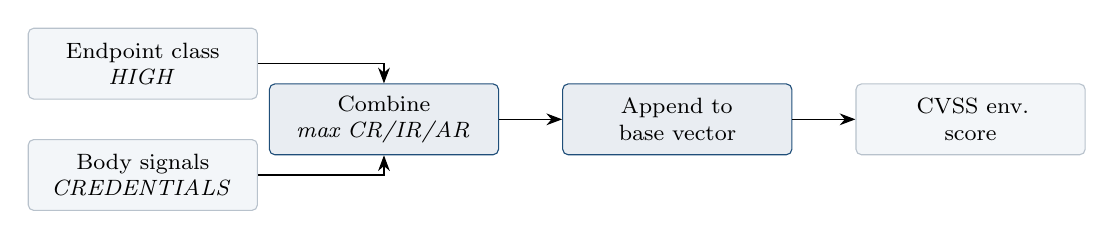
\begin{tikzpicture}[font=\footnotesize,>={Stealth[length=2mm]},
  s/.style={draw=rule,fill=soft,rounded corners=2pt,text width=27mm,align=center,minimum height=9mm,inner sep=3pt},
  d/.style={draw=brand,fill=brand!10},node distance=5mm and 8mm]
\node[s] (cls){Endpoint class\\\textit{HIGH}};
\node[s,below=5mm of cls] (sig){Body signals\\\textit{CREDENTIALS}};
\node[s,d,right=16mm of $(cls)!0.5!(sig)$] (max){Combine\\\textit{max CR/IR/AR}};
\node[s,d,right=of max] (vec){Append to\\base vector};
\node[s,right=of vec] (env){CVSS env.\\score};
\draw[->](cls)-|(max); \draw[->](sig)-|(max); \draw[->](max)--(vec); \draw[->](vec)--(env);
\end{tikzpicture}}
\end{center}

\textbf{Design decisions.} Using CVSS's own CR/IR/AR (not a custom weight) keeps
the output a standard, reproducible score. ``Max'' is deliberately
conservative: one strong reason to care (say, credentials in the body) is enough
to raise the requirement, rather than averaging it away. X for LOW means context
never \emph{lowers} a public finding below its base.
\textbf{Tested by} \texttt{make validate-config} and \texttt{tests/unit/test\_cvss.py}.
\textbf{Limitation:} the triples are expert judgement, defined once; they are not
learned from data.

\subsection{Sensitivity classifier}
\textbf{What it does.} \texttt{backend/app/ml/sensitivity.py} labels an endpoint
CRITICAL/HIGH/MEDIUM/LOW from the words in its path, so \texttt{cvss.py} knows
which class triple to use.

\textbf{How it works.} \texttt{classify(endpoint)} tokenises the path
(\texttt{path\_text()}), optionally expands abbreviations, and compares it with
class ``anchors'' using sentence-embedding similarity
(\texttt{AnchorClassifier}, config in \texttt{config/sensitivity\_anchors.yaml}).
Static assets short-circuit to LOW. When the ML packages or the anchor config are
absent, the engine falls back to Atta's built-in keyword classifier in
\texttt{core/sensitivity.py}.

\textbf{Design decision.} The semantic anchor classifier ships \emph{off by
default}; the keyword families are the default path. The anchor set scores
better on the evaluation (see Part C) but was kept optional to avoid a heavy
dependency in the default install. \textbf{Tested by} \texttt{tests/ml/} and the
sensitivity evaluation. \textbf{Limitation:} accuracy on a four-class problem is
modest (about 0.49 on the test split); the class boundaries are genuinely fuzzy.

\subsection{Response (body) classifier}
\textbf{What it does.} \texttt{backend/app/ml/body\_classifier.py} looks in a
response for sensitive data and returns a set of signals: CREDENTIALS, PII,
FINANCIAL, INTERNAL\_IP. Evidence is always redacted.

\textbf{How it works.} \texttt{analyze(response)} runs \texttt{detect()}, which
scans text (API-doc example blocks are stripped first) for credentials and
secret keys, personal data, financial numbers (validated with Luhn / IBAN
checks), and internal IPs. \texttt{shannon\_entropy()} and
\texttt{\_random\_looking()} help tell a real secret from a placeholder;
\texttt{mask()} redacts a value to its last few characters before it is stored.

\textbf{Design decision.} The classifier is conservative: placeholder and example
values are filtered so a documentation sample does not raise a real finding.
\textbf{Tested by} \texttt{tests/ml/} (fixtures of real-looking and placeholder
data). \textbf{Limitation:} it reads server responses only, so secrets rendered
by client-side JavaScript are not seen.

\subsection{Chain templates}
\textbf{What it does.} \texttt{config/chains.yaml} declares the five attack-chain
templates that Atta's \texttt{core/chains.py} correlates and scores.

\textbf{How it works.} Each template names the member checks, the scope they must
share, and a composite CVSS vector. The five are: session theft via XSS; error
disclosure plus version banner; credentialed CORS read on a sensitive API;
credential interception on login; and exposed configuration leaking live
credentials. \textbf{Tested by} \texttt{tests/unit/test\_chains.py}.
\textbf{Limitation:} a chain forms only where every member fires on the same
scope; on the evaluation targets chains appear only on DVWA and crAPI.

\subsection{The evaluation lab}
\textbf{What it does.} \texttt{eval/} is how the project proves itself: real
targets, a hand-written answer key, and a harness that scans with CAWASMA, ZAP
and Nuclei and scores all three.

\textbf{How it works.}
\begin{itemize}
\item \texttt{eval/ground\_truth/} holds, per target, which check should
(\texttt{present}) or should not (\texttt{absent}) fire on which endpoint: 33
present, 20 absent and 27 \texttt{must\_not\_fire} entries.
\item \texttt{harness/run\_all.py} resets the four targets, puts an HTTPS proxy
in front (so HTTPS-only CAWASMA can reach them), and scans with each tool.
\item \texttt{harness/evaluate.py} normalises each tool's output to CAWASMA check
ids (\texttt{tool\_mapping.yaml}), matches it to the answer key by target, check
and endpoint, and computes precision, recall and FPR. A tool is scored only on
the checks its rules can produce.
\item \texttt{harness/ranking.py} computes NDCG@10 for the base and the
context-aware ranking, averaged over 1000 random tie-breaks (seed 13).
\item \texttt{harness/final\_tables.py} writes the report tables in
\texttt{eval/results/final/}.
\end{itemize}

\textbf{Design decision.} Scoring is a set of pure functions over saved raw
output, so the metrics can be recomputed without re-scanning.
\textbf{Limitation:} the ground truth is one rater's first pass, and it uses
CAWASMA's own check ids, which favours CAWASMA's scope --- stated openly in the
write-up.

\section{Numbers to know}
All figures are from the repository at commit \texttt{7cc819f}.

\subsection{The mapping in action}
The same finding, scored on endpoints of each class, shows the mapping
working.\src{eval/results/final/mapping.md}
\begin{center}\small
\begin{tabular}{@{}lrrrrr@{}}
\toprule
Check & base & LOW & MEDIUM & HIGH & CRITICAL\\
\midrule
HDR-001 Missing HSTS & 5.3 & 5.3 & 5.3 & 7.1 & 7.1\\
HDR-007 Server banner & 5.3 & 5.3 & 5.3 & 6.1 & 6.1\\
\bottomrule
\end{tabular}
\end{center}
A public page keeps the base score; a login or admin endpoint is raised.

\subsection{Classifier accuracy, honestly}
Sensitivity classification is a hard four-class problem on 164 labelled
endpoints.\src{eval/results/final/classifier.md}
\begin{center}\small
\begin{tabular}{@{}llrrr@{}}
\toprule
Families & split & n & accuracy & macro F1\\
\midrule
shipped (keywords) & test & 113 & 0.425 & 0.362\\
proposed (anchors) & test & 113 & 0.487 & 0.454\\
proposed (anchors) & dev & 51 & 0.569 & 0.577\\
\bottomrule
\end{tabular}
\end{center}
The anchor set beats the keyword set, but accuracy is modest. The project does
not claim a strong classifier; it claims that a \emph{reasonable} class, combined
with body signals, moves scores in the right direction.

\subsection{Detection and ranking}
Detection (micro over four targets): CAWASMA recall 0.758, Nuclei 0.765, ZAP
0.333; all three precision 1.00.\src{eval/results/final/tools.md} Ranking
(NDCG@10, environmental findings, base $\rightarrow$ context): mean $0.324
\rightarrow 0.347$; better than base only on DVWA
($0.147\rightarrow0.261$).\src{eval/results/final/ranking\_environmental.md}
The graded pools are not finished, so there is no pool-based NDCG yet.

\section{Contribution timeline}
Grouped from merged pull requests.\src{gh pr list (upstream); git log}
\begin{center}\small
\begin{tabularx}{\linewidth}{@{}llX@{}}
\toprule
Merged & PRs & What changed\\
\midrule
25 Oct & \#8, \#11 & Set up the ML and evaluation workspace; evaluation setup.\\
25 Oct & \#9, \#18 & Draft passive check specifications; check ids.\\
25 Oct & \#10, \#19 & Environmental CVSS context mapping; mapping demo uses the real vectors.\\
25 Oct & \#17 & Pin \texttt{preshed} so spaCy loads; ML smoke test.\\
25 Oct & \#20 & Chains format 1.1: groups, scope, context, composite vectors.\\
27 Oct & \#37 & Evaluation ground truth.\\
27 Oct & \#38 & Response (body) classifier.\\
27 Oct & \#40 & Evaluation harness.\\
4 Nov & \#49 & Final evaluation, ranking experiment, tuning, security signatures.\\
\bottomrule
\end{tabularx}
\end{center}
\textbf{Reviews received.} Atta pushed fixes inside Asim's files on
\texttt{atta/fix-asim-*} branches for Asim to review: catalog vectors (\#58),
the five check specs (\#56), the sensitivity anchors (\#60), the ranking
experiment (\#61), fake-secret values (\#62), spec approval (\#70), formatting
(\#71) and the refreshed pools (\#72).

\section{Viva preparation}
\subsection{Likely questions, with short answers}
\begin{enumerate}[leftmargin=*,itemsep=3pt]
\item \textbf{Your ground truth uses your own check ids --- isn't that biased?}
Yes, and the write-up says so. It favours CAWASMA's scope, so ZAP and Nuclei are
scored only on the checks their rules map to (``not covered'' counts the rest).
\item \textbf{Why CVSS environmental metrics and not your own weighting?} Because
the output is then a standard score anyone can reproduce; only the mapping to
CR/IR/AR is ours, and it is a short, auditable table.
\item \textbf{Why ``max'' to combine class and signals?} It is conservative: one
strong reason to care is enough to raise a requirement. Averaging would let a
single public-looking token hide a real credential leak.
\item \textbf{Why does LOW map to X/X/X?} X is ``Not Defined'', the neutral
baseline. A public endpoint should keep its base score; context raises scores, it
does not lower public ones.
\item \textbf{The ranking isn't better overall --- what does the project prove?}
It proves the mechanism: on a sensitive, credential-bearing endpoint the same
weakness scores higher, with a reproducible vector. The ranking study is honest
that, on four targets, it is not better overall, and the pools are ungraded.
\item \textbf{Your classifier accuracy is under 0.5 --- is that good enough?}
For a fuzzy four-class problem it is modest but usable; the score moves in the
right direction because body signals back up the class. We do not oversell it.
\item \textbf{How do you avoid flagging example data as a real secret?} The body
classifier strips API-doc example blocks and filters placeholder values, and uses
entropy to tell a real secret from a dummy.
\item \textbf{How is a credit-card number confirmed?} With a Luhn check; IBANs
with an IBAN check. A number that fails the check is not reported as financial
data.
\item \textbf{Why is the anchor classifier off by default?} To keep the default
install light; the keyword classifier needs no model. The anchor set is the
better, optional path.
\item \textbf{How do you compare fairly with ZAP and Nuclei?} Each tool's rules
are mapped to check ids; each is scored only on what it can report; the endpoint
match is strict; false positives count only against explicit \texttt{absent}
entries.
\item \textbf{Why did ZAP do so poorly?} It ran in passive baseline mode, which
by design makes no attacks; these numbers do not represent a full active ZAP
scan.
\item \textbf{What is NDCG@10 and why 1000 tie-breaks?} It scores how well a
ranking puts graded items near the top; base scores tie a lot, so the result is
averaged over 1000 random orderings of ties with a fixed seed.
\item \textbf{What are the five attack chains?} Session theft via XSS; error plus
version banner; credentialed CORS read; credential interception on login; exposed
config leaking credentials.
\item \textbf{How many ground-truth entries are there?} 33 present, 20 absent and
27 must-not-fire, across four targets --- too few for a significance claim.
\item \textbf{Where does a check's base score come from?} The fixed CVSS v3.1
base vector in the catalog, not the catalog's \texttt{base\_score} field (31
disagree; the vector wins).
\item \textbf{How does the engine keep working without your ML code?} Through the
contract in \texttt{app/core/contracts.py}: the built-in keyword and regex
classifiers are the fallback.
\item \textbf{Could the mapping be learned instead of hand-set?} In principle,
with far more labelled data; today it is expert judgement, which is defensible
and transparent.
\item \textbf{What stops a check specification from breaking the engine?}
\texttt{make validate-config} checks every vector parses and matches
\texttt{checks.yaml} before it can be used.
\item \textbf{How do you redact evidence?} \texttt{mask()} keeps only the last few
characters; redaction also runs again on every export.
\item \textbf{What is the biggest threat to your evaluation's validity?} The
single-rater ground truth and the small target count; both are stated as
limitations.
\item \textbf{Why these four targets?} Juice Shop, DVWA, VAmPI and crAPI are
well-known, intentionally vulnerable apps that between them cover web pages and
REST APIs, so the ground truth can be written with confidence.
\item \textbf{Why keep a legacy formula at all?} Not every check has a reviewed
spec yet; the 37 legacy checks keep working under the interim formula and migrate
to the environmental path one at a time.
\item \textbf{How does a sensitivity class become a number?} Its CR/IR/AR triple
is appended to the check's base vector and the \texttt{cvss} library computes the
environmental score; nothing else changes.
\item \textbf{What does ``not covered'' mean in the comparison?} Ground-truth
entries for checks a tool has no rule for; they are listed, not counted as misses,
so the tool is judged only on what it can report.
\item \textbf{What would make the ranking result stronger?} Grading the priority
pools (for a pool-based NDCG), more targets, and a second rater verifying the
ground truth.
\item \textbf{How are abbreviations in a path handled?} \texttt{path\_text()} can
expand them (optionally with an LLM step) before the class is decided, so
\texttt{/acct} and \texttt{/account} read alike.
\item \textbf{Is any of your scoring machine-learned?} The classifiers use
embeddings, but the CR/IR/AR mapping is a fixed, human-set table --- which is why
the final score stays explainable.
\end{enumerate}

\subsection{Three-minute demo script}
\begin{enumerate}[leftmargin=*]
\item Open \texttt{cvss\_mapping.yaml}. Say: ``Class and signals become CR/IR/AR;
the highest wins; LOW is X so public pages keep their base.''
\item Show a HIGH finding's detail in the app: base 5.3, final 7.1, with the
vector. Say: ``Standard CVSS environmental maths.''
\item Run \texttt{make coverage-stats}. Point at 25 environmental vs 37 legacy.
\item Show \texttt{eval/results/final/tools.md} and \texttt{ranking\_environmental.md}.
Say the honest ranking result out loud.
\item Show \texttt{classifier.md}. Say: ``Anchors beat keywords; accuracy is
modest and we say so.''
\end{enumerate}

\subsection{Five things to explain without notes}
\begin{enumerate}[leftmargin=*]
\item The mapping: class + signals $\rightarrow$ CR/IR/AR, combine by max, LOW=X.
\item Why a fixed base vector per check, and that only context is ours.
\item How the evaluation scores a tool only on the checks it can report.
\item The honest ranking and classifier numbers, and what they do and do not show.
\item The body classifier's placeholder/entropy filtering and redaction.
\end{enumerate}

% Part F: glossary. Shared, identical in all three documents.
\section{Glossary}
\begin{description}[leftmargin=0pt,style=nextline,itemsep=3pt]
\item[CVSS base score] The standard severity of a vulnerability on its own, 0--10,
from a vector such as \texttt{AV:N/AC:L/\dots}. Fixed per check; never invented per scan.
\item[CVSS environmental score] The base score recomputed for a particular
environment, using CR/IR/AR and modified base metrics. CAWASMA's context-aware
score is this.
\item[CR / IR / AR] Confidentiality, Integrity and Availability \emph{Requirements}:
environmental inputs saying how much each property matters here. Values Low,
Medium, High, or X (Not Defined). CAWASMA sets them from the endpoint class and
the data in the response.
\item[Sensitivity class] CAWASMA's label for how sensitive an endpoint is ---
CRITICAL, HIGH, MEDIUM or LOW --- from the words in its URL path.
\item[Body signals] Sensitive data found in a response: credentials, personal
data (PII), financial data, or an internal IP address. Evidence is redacted.
\item[Base vs.\ final score] CAWASMA always keeps both: the official base score
and the context-aware (environmental) final score, in separate columns.
\item[Legacy vs.\ environmental scoring] A finding is scored either by the CVSS
environmental metrics (approved specs) or by the interim legacy formula; its
\texttt{scoring\_method} says which.
\item[Precision] Of the findings that were judged, the fraction that were
correct: $\text{TP}/(\text{TP}+\text{FP})$.
\item[Recall] Of the real issues in the answer key, the fraction found:
$\text{TP}/(\text{TP}+\text{FN})$.
\item[FPR] False-positive rate: $\text{FP}/(\text{FP}+\text{TN})$.
\item[Ground truth] A hand-written list, per target, of which check should
(\texttt{present}) or should not (\texttt{absent}) fire on which endpoint.
\item[NDCG@10] Normalised Discounted Cumulative Gain at rank 10: a score for how
well a ranking puts the important items near the top, against a graded list.
\item[Tie-break sampling] Base scores tie often, so a ranking's NDCG is averaged
over 1000 random orderings of the tied items, with a fixed seed.
\item[SSRF] Server-Side Request Forgery: tricking the scanner into requesting an
internal address. CAWASMA guards against it by validating the resolved IP on
every hop.
\item[Soft-404] A page that returns HTTP 200 but is really ``not found''. The
crawler learns a baseline so it does not treat these as real endpoints.
\item[Passive vs.\ active scan] Passive sends only safe GET/HEAD and reads what
comes back; active sends extra, still non-destructive, probes. CAWASMA never
sends attack payloads.
\item[BOLA / IDOR] Broken Object-Level Authorisation / Insecure Direct Object
Reference: reading another user's object by changing an id. CAWASMA only flags an
\emph{indicator}; confirming it needs logged-in accounts, which is future work.
\item[Attack chain] Several findings that together make a bigger risk, correlated
from a template and scored with their own composite vector.
\item[Environmental metric ``X''] ``Not Defined'': the neutral baseline. A public
(LOW) endpoint uses X, so its score is unchanged --- context only ever raises a
score here, it does not lower a public page below its base.
\end{description}

\end{document}
